\documentclass[12pt]{article}

\usepackage{amsmath}
\usepackage{amsthm}
\usepackage{amssymb}
\usepackage{mathrsfs}
\usepackage{setspace}
\usepackage{graphicx}
\usepackage{caption}
\usepackage{subcaption}
\usepackage{minted}

\newcommand{\w}{\omega}
\renewcommand{\a}{\alpha}
\renewcommand{\d}{\delta}
\newcommand{\s}{\sigma}
\newcommand{\e}{\epsilon}
\newcommand{\m}{\mu}

\newcommand{\inn}[1]{\left\langle #1 \right\rangle}
\newcommand{\norm}[1]{\left\Vert #1 \right\Vert}
\newcommand{\abs}[1]{\left\vert #1 \right\vert}

\newcommand{\real}{\mathbb{R}}
\newcommand{\nat}{\mathbb{Z}^+}

\begin{document}

\title{Homework 5}
\date{\today}
\author{Hunter Schwartz}
\maketitle

%\doublespacing

\textbf{Problem 0}

The correction I made is in line $29$ of the rk4 code, in the calculation of the K4 coefficient, the error having potentially come from copy/pasting without changing some subtly different variables.

\begin{minted}[frame=lines,fontsize=\footnotesize,linenos]{python}
def rk4(f,t0,y0,h,m):

    b21 = 1/2
    b31 = 0
    b32 = 3/4
    b41 = 2/9
    b42 = 0
    b43 = 1/3
    b51 = 1/6
    b52 = 1/3
    b53 = 1/3
    b54 = 1/6
        
    t = t0
    y = np.array(y0)

    ya = np.empty((len(y0),m+1))
    ya[:,0] = y
    ta = np.linspace(t0,t0+m*h,m+1)
     
    for k in range(m):
        t = t0 + k*h
        K1 = f(t,y)  
        y1 = y + h*b21*K1
        K2 = f(t+h*b21,y1)
        y2 = y + h*(b31*K1 + b32*K2)
        K3 = f(t+h*(b31    + b32   ), y2)
        y3 = y + h*(b41*K1 + b42*K2 + b43*K3)
        #K4 = f(t+h*(b31    + b32    + b43   ), y3)
        K4 = f(t+h*(b41    + b42    + b43   ), y3)
        y4 = y + h*(b51*K1 + b52*K2 + b53*K3 + b54*K4)
        y = y4
        ya[:,k+1] = y
        
    return ta,ya
\end{minted}

\newpage

\textbf{Problem 1}

(a) The code to solve the problem from class is reprinted below. 

\begin{minted}[frame=lines,fontsize=\footnotesize,linenos]{python}
import numpy as np

def rk4(f,t0,y0,h,m):

    b21 = 1/2
    b31 = 0
    b32 = 3/4
    b41 = 2/9
    b42 = 0
    b43 = 1/3
    b51 = 1/6
    b52 = 1/3
    b53 = 1/3
    b54 = 1/6
        
    t = t0
    y = np.array(y0)

    ya = np.empty((len(y0),m+1))
    ya[:,0] = y
    ta = np.linspace(t0,t0+m*h,m+1)
     
    for k in range(m):
        t = t0 + k*h
        K1 = f(t,y)  
        y1 = y + h*b21*K1
        K2 = f(t+h*b21,y1)
        y2 = y + h*(b31*K1 + b32*K2)
        K3 = f(t+h*(b31    + b32   ), y2)
        y3 = y + h*(b41*K1 + b42*K2 + b43*K3)
        #K4 = f(t+h*(b31    + b32    + b43   ), y3)
        K4 = f(t+h*(b41    + b42    + b43   ), y3)
        y4 = y + h*(b51*K1 + b52*K2 + b53*K3 + b54*K4)
        y = y4
        ya[:,k+1] = y
        
    return ta,ya
    
def f(x,Y):
    global p,q,phi
    y,yp = Y
    return np.array([ yp, phi(x) -p(x)*yp - q(x)*y ])
    
def p(x):   return 5*x**2
def q(x):   return 30+50*np.sin(30*x)
def phi(x): return 50*np.cosh(x)
x0,x1 = 0,1
alpha = 1
beta = 10
y0 = alpha

m = 501
h = (x1-x0)/m

sa = np.array([0,50])
y1a = np.empty(2)

for i, sigma in enumerate(sa):
    ta,Ya = rk4(f,x0,[y0,sigma],h,m)
    plt.plot(ta,Ya[0,:])
    y1a[i] = Ya[0,-1]
    
rho = (beta - y1a[0]) / (y1a[1] - y1a[0])
s3 = sa[0] + rho*(sa[1] - sa[0])             # Slope to hit desired target
ta,Ya = rk4(f,x0,[y0,s3],h,m)                # Solution to BVP
\end{minted}

The plot of exploratory shots and solution is included below. \\

\begin{figure}[h]
\centering
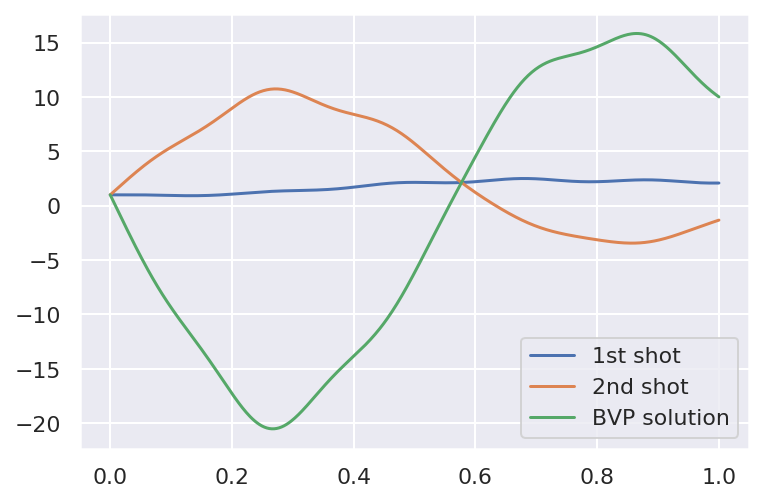
\includegraphics[width=.8\textwidth]{p1.png}
\caption{Solutions for various initial slopes; $1$st shot: $0$, $2$nd shot: $50$, $3$rd shot as calculated.}
\end{figure}

\newpage 

This results in the following estimates, truncated at $8$ decimal places: \\

\begin{align*}
y'(0) = -116.08319842 \\
y(0.2) = -17.39286367 \\
y(1) = 9.99999999
\end{align*}

\newpage

\textbf{Problem 2}

\begin{minted}[frame=lines,fontsize=\footnotesize,linenos]{python}
import numpy as np

def rk4(f,t0,y0,h,m):

    b21 = 1/2
    b31 = 0
    b32 = 3/4
    b41 = 2/9
    b42 = 0
    b43 = 1/3
    b51 = 1/6
    b52 = 1/3
    b53 = 1/3
    b54 = 1/6
        
    t = t0
    y = np.array(y0)

    ya = np.empty((len(y0),m+1))
    ya[:,0] = y
    ta = np.linspace(t0,t0+m*h,m+1)
     
    for k in range(m):
        t = t0 + k*h
        K1 = f(t,y)  
        y1 = y + h*b21*K1
        K2 = f(t+h*b21,y1)
        y2 = y + h*(b31*K1 + b32*K2)
        K3 = f(t+h*(b31    + b32   ), y2)
        y3 = y + h*(b41*K1 + b42*K2 + b43*K3)
        #K4 = f(t+h*(b31    + b32    + b43   ), y3)
        K4 = f(t+h*(b41    + b42    + b43   ), y3)
        y4 = y + h*(b51*K1 + b52*K2 + b53*K3 + b54*K4)
        y = y4
        ya[:,k+1] = y
        
    return ta,ya
    
def f(t,Y):
    x,y,z = Y
    return np.array([10*y - 10*x,
                    28*x - y - x*z,
                    -8/3*z + x*y])

def Df(t,Y):
    x,y,z = Y
    return np.array([[-10, 10, 0],
                    [28 - z, -1, -x],
                    [y, x, -8/3]])

def Vp(t,Y,V):
    return np.matmul( Df(t,Y), V )

V0 = np.eye(3)
Y0 = np.array([-5, -8, 15])

def dZ(t,Z):
    V = Z[:-3].reshape((3,3))
    Y = Z[-3:]
    dV = Vp(t,Y,V)
    dY = f(t,Y)
    return np.append(dV.reshape(-1,1), dY)

Z0 = np.append(V0.reshape(-1,1), Y0)
t0 = 0
tf = 10.8
m = 10**5

h = (tf - t0)/m
ta,Ya = rk4(dZ,t0,Z0,h,m)
xa,ya,za = Ya[-3:,:]
\end{minted}

A plot of part of the solution is included for reference below.
\\

\begin{figure}[h]
\centering
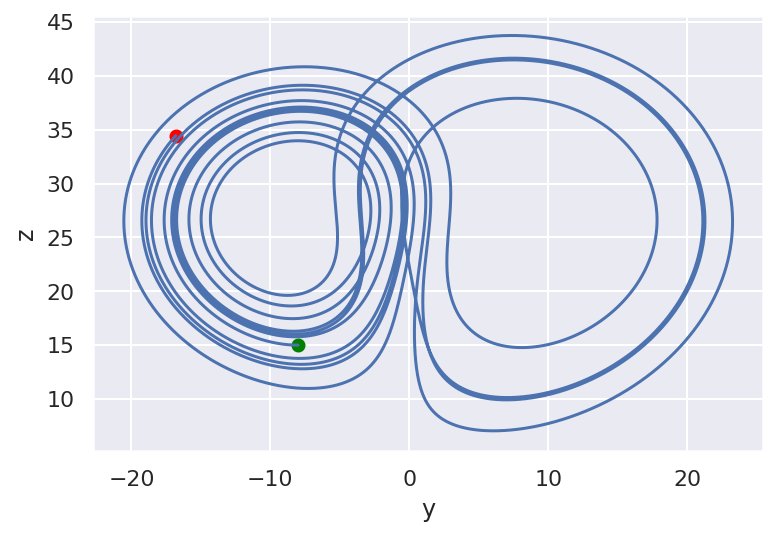
\includegraphics[width=.8\textwidth]{p2.png}
\caption{Solution to Lorenz equation, inital condition (green) and solution at ending time (red) indicated.}
\end{figure}

From this, we get

\begin{align*}
V(10.8) =
\begin{bmatrix}
765.005 & -402.375 & -2779.392 \\
-21340.573 & 11230.615 & 77546.916 \\
-24387.797 & 12833.677 & 88618.627
\end{bmatrix},
\end{align*}

with singular values $\s_1 = 1.233\times10^5$, $\s_2 = 3.8238\times10^{-1}$, and $\s_3 = 6.6589\times10^{-13}$.
\\

\newpage

(b) In our case, these singular values can be thought of as representing the degree to which $Y(10.8)$ changes under perturbations in $Y(0)$. In particular, $s_1 = 1.233\times10^5$ denotes that there is a direction in which we can push $Y(0)$ that can cause approximately $5$ orders of magnitude larger a change in the value of $Y(10.8)$. This is the singular value responsible for the chaotic behavior of the system. Small changes in $Y(0)$ along the direction associated with $\sigma_2 = 3.8238\times10^{-1}$ results in a change of roughly comparable size in the value of $Y(10.8)$, and small changes in the direction associated with $\s_3 = 6.6589\times10^{-13}$ will have essentially no influence on the value of $Y(10.8)$.

\end{document}